\begin{figure*}
    \centering
    \begin{subfigure}{0.45\linewidth}
        \centering
        \begin{adjustbox}{width=\textwidth}
            % This file was created by tikzplotlib v0.9.5.
\begin{tikzpicture}







\begin{axis}[
axis background/.style={fill=white!89.8039215686275!black},
axis line style={white},
legend cell align={left},
legend style={fill opacity=0.8, draw opacity=1, text opacity=1, at={(0.03,0.97)}, anchor=north west, draw=white!80!black, fill=white!89.8039215686275!black},
log basis y={10},
tick align=outside,
tick pos=left,
title={Average sample time for batch size $=32$},
x grid style={white},
xlabel={resolution},
xmajorgrids,
xmin=2.65, xmax=10.35,
xtick style={color=white!33.3333333333333!black},
y grid style={white},
ylabel={time [ms]},
ymajorgrids,
ymin=0.152640394088257, ymax=27.8442975883733,
ymode=log,
ytick style={color=white!33.3333333333333!black},
xticklabels={$2^3$, $2^4$, $2^5$, $2^6$, $2^7$, $2^8$, $2^9$, $2^{10}$},
xtick={3,...,10},
]
\path [fill=cudnn, fill opacity=0.2, very thin]
(axis cs:3,0.201026)
--(axis cs:3,0.19947)
--(axis cs:4,0.199807)
--(axis cs:5,0.227339)
--(axis cs:6,0.330417)
--(axis cs:7,0.861158)
--(axis cs:8,2.71924)
--(axis cs:8,2.77216)
--(axis cs:8,2.77216)
--(axis cs:7,0.88903)
--(axis cs:6,0.3433)
--(axis cs:5,0.230137)
--(axis cs:4,0.204628)
--(axis cs:3,0.201026)
--cycle;

\path [fill=libtorch, fill opacity=0.2, very thin]
(axis cs:3,0.239017)
--(axis cs:3,0.224985)
--(axis cs:4,0.223488)
--(axis cs:5,0.227935)
--(axis cs:6,0.260423)
--(axis cs:7,0.475671)
--(axis cs:8,1.50341)
--(axis cs:9,5.67418)
--(axis cs:9,5.86691)
--(axis cs:9,5.86691)
--(axis cs:8,1.56544)
--(axis cs:7,0.483492)
--(axis cs:6,0.261208)
--(axis cs:5,0.242581)
--(axis cs:4,0.238601)
--(axis cs:3,0.239017)
--cycle;

\path [fill=pytorch, fill opacity=0.2, very thin]
(axis cs:3,1.264947)
--(axis cs:3,1.21564)
--(axis cs:4,1.213545)
--(axis cs:5,1.215587)
--(axis cs:6,1.220171)
--(axis cs:7,1.296469)
--(axis cs:8,2.795173)
--(axis cs:9,9.585992)
--(axis cs:9,9.846071)
--(axis cs:9,9.846071)
--(axis cs:8,2.891976)
--(axis cs:7,1.341868)
--(axis cs:6,1.291262)
--(axis cs:5,1.29437)
--(axis cs:4,1.259168)
--(axis cs:3,1.264947)
--cycle;

\path [fill=white!46.6666666666667!black, fill opacity=0.2, very thin]
(axis cs:3,0.353049)
--(axis cs:3,0.199058)
--(axis cs:4,0.193395)
--(axis cs:5,0.195655)
--(axis cs:6,0.227985)
--(axis cs:7,0.435408)
--(axis cs:8,1.42414)
--(axis cs:9,5.45931)
--(axis cs:10,20.8873)
--(axis cs:10,21.9766)
--(axis cs:10,21.9766)
--(axis cs:9,5.7139)
--(axis cs:8,1.5859)
--(axis cs:7,0.616575)
--(axis cs:6,0.401246)
--(axis cs:5,0.348112)
--(axis cs:4,0.374466)
--(axis cs:3,0.353049)
--cycle;

\path [fill=torchscript, fill opacity=0.2, very thin]
(axis cs:3,0.353049)
--(axis cs:3,0.199058)
--(axis cs:4,0.193395)
--(axis cs:5,0.195655)
--(axis cs:6,0.227985)
--(axis cs:7,0.435408)
--(axis cs:8,1.42414)
--(axis cs:9,5.45931)
--(axis cs:10,20.8873)
--(axis cs:10,21.9766)
--(axis cs:10,21.9766)
--(axis cs:9,5.7139)
--(axis cs:8,1.5859)
--(axis cs:7,0.616575)
--(axis cs:6,0.401246)
--(axis cs:5,0.348112)
--(axis cs:4,0.374466)
--(axis cs:3,0.353049)
--cycle;

\addplot [semithick, cudnn]
table {%
3 0.200238913297653
4 0.202598989009857
5 0.229123681783676
6 0.338942557573318
7 0.870264947414398
8 2.73578190803528
};
\addlegendentry{cudnn}
\addplot [semithick, libtorch]
table {%
3 0.232446998357773
4 0.230680495500565
5 0.237425118684769
6 0.260794192552567
7 0.47879546880722
8 1.53802895545959
9 5.7626690864563
};
\addlegendentry{libtorch}
\addplot [semithick, pytorch]
table {%
3 1.23768603801727
4 1.23296797275543
5 1.24600088596344
6 1.25468814373016
7 1.31825852394104
8 2.83480596542358
9 9.69671154022217
};
\addlegendentry{pytorch}
\addplot [semithick, torchscript]
table {%
3 0.220640391111374
4 0.216945394873619
5 0.211528897285461
6 0.245379000902176
7 0.460912704467773
8 1.45570909976959
9 5.53999090194702
10 21.3651218414307
};
\addlegendentry{torchscript}
\end{axis}

\end{tikzpicture}

        \end{adjustbox}
        \label{fig:avg_sample_time_32}
    \end{subfigure}%
    \begin{subfigure}{0.45\textwidth}
        \centering
        \begin{adjustbox}{width=\textwidth}
            % This file was created by tikzplotlib v0.9.5.
\begin{tikzpicture}







\begin{axis}[
axis background/.style={fill=white!89.8039215686275!black},
axis line style={white},
%legend cell align={left},
%legend style={fill opacity=0.8, draw opacity=1, text opacity=1, draw=white!80!black, fill=white!89.8039215686275!black},
log basis y={10},
tick align=outside,
tick pos=left,
title={Average sample time for resolution $=64$},
x grid style={white},
xlabel={batch size},
xmajorgrids,
xmin=2.7, xmax=9.3,
xtick style={color=white!33.3333333333333!black},
y grid style={white},
%ylabel={time [ms]},
ymajorgrids,
ymin=0.0318818812180445, ymax=4.24381955156468,
ymode=log,
ytick style={color=white!33.3333333333333!black},
xticklabels={$2^3$, $2^4$, $2^5$, $2^6$, $2^7$, $2^8$, $2^9$},
xtick={3,...,9},
]
\path [fill=cudnn, fill opacity=0.2, very thin]
(axis cs:3,0.532711)
--(axis cs:3,0.525274)
--(axis cs:4,0.325467)
--(axis cs:5,0.227339)
--(axis cs:6,0.137164)
--(axis cs:7,0.127286)
--(axis cs:8,0.107328)
--(axis cs:9,0.0943382)
--(axis cs:9,0.100206)
--(axis cs:9,0.100206)
--(axis cs:8,0.1119)
--(axis cs:7,0.129387)
--(axis cs:6,0.145102)
--(axis cs:5,0.230137)
--(axis cs:4,0.333086)
--(axis cs:3,0.532711)
--cycle;

\path [fill=libtorch, fill opacity=0.2, very thin]
(axis cs:3,0.7206)
--(axis cs:3,0.643425)
--(axis cs:4,0.371694)
--(axis cs:5,0.227935)
--(axis cs:6,0.138768)
--(axis cs:7,0.110285)
--(axis cs:8,0.0866569)
--(axis cs:9,0.0769451)
--(axis cs:9,0.077837)
--(axis cs:9,0.077837)
--(axis cs:8,0.0870269)
--(axis cs:7,0.110558)
--(axis cs:6,0.149246)
--(axis cs:5,0.242581)
--(axis cs:4,0.39549)
--(axis cs:3,0.7206)
--cycle;

\path [fill=pytorch, fill opacity=0.2, very thin]
(axis cs:3,3.397831)
--(axis cs:3,3.123268)
--(axis cs:4,2.145072)
--(axis cs:5,1.215587)
--(axis cs:6,0.90215)
--(axis cs:7,0.489502)
--(axis cs:8,0.516421)
--(axis cs:9,0.290157)
--(axis cs:9,0.314908)
--(axis cs:9,0.314908)
--(axis cs:8,0.564356)
--(axis cs:7,0.522439)
--(axis cs:6,1.003318)
--(axis cs:5,1.29437)
--(axis cs:4,2.273831)
--(axis cs:3,3.397831)
--cycle;

\path [fill=white!46.6666666666667!black, fill opacity=0.2, very thin]
(axis cs:3,0.797093)
--(axis cs:3,0.633669)
--(axis cs:4,0.342584)
--(axis cs:5,0.195655)
--(axis cs:6,0.101828)
--(axis cs:7,0.071068)
--(axis cs:8,0.0474417)
--(axis cs:9,0.0398198)
--(axis cs:9,0.13526)
--(axis cs:9,0.13526)
--(axis cs:8,0.145412)
--(axis cs:7,0.180774)
--(axis cs:6,0.20295)
--(axis cs:5,0.348112)
--(axis cs:4,0.497252)
--(axis cs:3,0.797093)
--cycle;

\path [fill=torchscript, fill opacity=0.2, very thin]
(axis cs:3,0.797093)
--(axis cs:3,0.633669)
--(axis cs:4,0.342584)
--(axis cs:5,0.195655)
--(axis cs:6,0.101828)
--(axis cs:7,0.071068)
--(axis cs:8,0.0474417)
--(axis cs:9,0.0398198)
--(axis cs:9,0.13526)
--(axis cs:9,0.13526)
--(axis cs:8,0.145412)
--(axis cs:7,0.180774)
--(axis cs:6,0.20295)
--(axis cs:5,0.348112)
--(axis cs:4,0.497252)
--(axis cs:3,0.797093)
--cycle;

\addplot [semithick, cudnn]
table {%
3 0.527113080024719
4 0.328776597976685
5 0.229123681783676
6 0.139674320816994
7 0.128557801246643
8 0.10912749171257
9 0.098616324365139
};
%\addlegendentry{cudnn}
\addplot [semithick, libtorch]
table {%
3 0.66579794883728
4 0.376946628093719
5 0.237425118684769
6 0.141885712742805
7 0.110373191535473
8 0.0867782235145569
9 0.077290840446949
};
%\addlegendentry{libtorch}
\addplot [semithick, pytorch]
table {%
3 3.20224666595459
4 2.2035346031189
5 1.24600088596344
6 0.938888311386108
7 0.50709193944931
8 0.551432967185974
9 0.300852745771408
};
%\addlegendentry{pytorch}
\addplot [semithick, torchscript]
table {%
3 0.662334620952606
4 0.360176265239716
5 0.211528897285461
6 0.112016521394253
7 0.0824229493737221
8 0.0573519766330719
9 0.0495683811604977
};
%\addlegendentry{torchscript}
\end{axis}

\end{tikzpicture}

        \end{adjustbox}
    \end{subfigure}
    \\
    \begin{subfigure}{0.45\textwidth}
        \centering
        \begin{adjustbox}{width=\textwidth}
            % This file was created by tikzplotlib v0.9.5.
\begin{tikzpicture}







\begin{axis}[
axis background/.style={fill=white!89.8039215686275!black},
axis line style={white},
%legend cell align={left},
%legend style={fill opacity=0.8, draw opacity=1, text opacity=1, at={(0.03,0.97)}, anchor=north west, draw=white!80!black, fill=white!89.8039215686275!black},
log basis y={10},
tick align=outside,
tick pos=left,
title={Average used memory for batch size $=32$},
x grid style={white},
xlabel={resolution},
xmajorgrids,
xmin=2.65, xmax=10.35,
xtick style={color=white!33.3333333333333!black},
y grid style={white},
ylabel={memory [MB]},
ymajorgrids,
ymin=981.538600682435, ymax=24927.29576095,
ymode=log,
ytick style={color=white!33.3333333333333!black},
xticklabels={$2^3$, $2^4$, $2^5$, $2^6$, $2^7$, $2^8$, $2^9$, $2^{10}$},
xtick={3,...,10},
]
\path [fill=cudnn, fill opacity=0.2, very thin]
(axis cs:3,1137)
--(axis cs:3,1137)
--(axis cs:4,1161)
--(axis cs:5,1291)
--(axis cs:6,1853)
--(axis cs:7,3819)
--(axis cs:8,11683)
--(axis cs:8,11683)
--(axis cs:8,11683)
--(axis cs:7,3819)
--(axis cs:6,1853)
--(axis cs:5,1291)
--(axis cs:4,1161)
--(axis cs:3,1137)
--cycle;

\path [fill=libtorch, fill opacity=0.2, very thin]
(axis cs:3,1559)
--(axis cs:3,1559)
--(axis cs:4,1567)
--(axis cs:5,1613)
--(axis cs:6,1785)
--(axis cs:7,2529)
--(axis cs:8,5591)
--(axis cs:9,18415)
--(axis cs:9,18417)
--(axis cs:9,18417)
--(axis cs:8,5591)
--(axis cs:7,2529)
--(axis cs:6,1785)
--(axis cs:5,1613)
--(axis cs:4,1567)
--(axis cs:3,1559)
--cycle;

\path [fill=pytorch, fill opacity=0.2, very thin]
(axis cs:3,1529)
--(axis cs:3,1529)
--(axis cs:4,1539)
--(axis cs:5,1583)
--(axis cs:6,1799)
--(axis cs:7,2667)
--(axis cs:8,6473)
--(axis cs:9,21519)
--(axis cs:9,21519)
--(axis cs:9,21519)
--(axis cs:8,6473)
--(axis cs:7,2667)
--(axis cs:6,1799)
--(axis cs:5,1583)
--(axis cs:4,1539)
--(axis cs:3,1529)
--cycle;

\path [fill=white!46.6666666666667!black, fill opacity=0.2, very thin]
(axis cs:3,1357)
--(axis cs:3,1357)
--(axis cs:4,1357)
--(axis cs:5,1359)
--(axis cs:6,1379)
--(axis cs:7,1459.02)
--(axis cs:8,1849.85)
--(axis cs:9,3454.26)
--(axis cs:10,9872.04)
--(axis cs:10,9891)
--(axis cs:10,9891)
--(axis cs:9,3459)
--(axis cs:8,1855)
--(axis cs:7,1461)
--(axis cs:6,1379)
--(axis cs:5,1359)
--(axis cs:4,1357)
--(axis cs:3,1357)
--cycle;

\path [fill=torchscript, fill opacity=0.2, very thin]
(axis cs:3,1357)
--(axis cs:3,1357)
--(axis cs:4,1357)
--(axis cs:5,1359)
--(axis cs:6,1379)
--(axis cs:7,1459.02)
--(axis cs:8,1849.85)
--(axis cs:9,3454.26)
--(axis cs:10,9872.04)
--(axis cs:10,9891)
--(axis cs:10,9891)
--(axis cs:9,3459)
--(axis cs:8,1855)
--(axis cs:7,1461)
--(axis cs:6,1379)
--(axis cs:5,1359)
--(axis cs:4,1357)
--(axis cs:3,1357)
--cycle;

\addplot [semithick, cudnn]
table {%
3 1136.99975585938
4 1161
5 1290.99975585938
6 1853
7 3819.00048828125
8 11683.0029296875
};
%\addlegendentry{cudnn}
\addplot [semithick, libtorch]
table {%
3 1558.99975585938
4 1567.00024414062
5 1613.00024414062
6 1784.99975585938
7 2529.00024414062
8 5590.99951171875
9 18416.791015625
};
%\addlegendentry{libtorch}
\addplot [semithick, pytorch]
table {%
3 1529
4 1539.00024414062
5 1583.00036621094
6 1798.99975585938
7 2667
8 6472.998046875
9 21519.01171875
};
%\addlegendentry{pytorch}
\addplot [semithick, torchscript]
table {%
3 1356.99987792969
4 1356.99987792969
5 1359.00012207031
6 1379
7 1460.80187988281
8 1854.48486328125
9 3458.5263671875
10 9889.10546875
};
%\addlegendentry{torchscript}
\end{axis}

\end{tikzpicture}

        \end{adjustbox}
    \end{subfigure}
    \begin{subfigure}{0.45\textwidth}
        \centering
        \begin{adjustbox}{width=\textwidth}
            % This file was created by tikzplotlib v0.9.5.
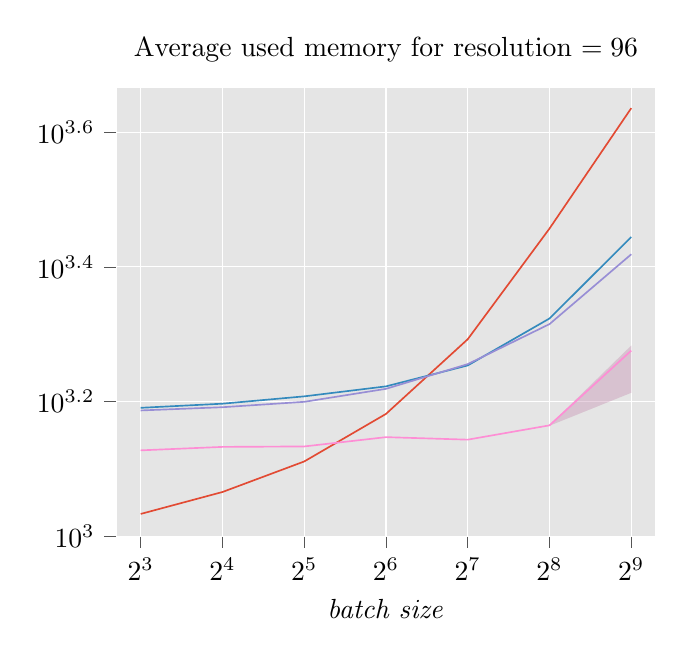
\begin{tikzpicture}

\definecolor{color0}{rgb}{0.886274509803922,0.290196078431373,0.2}
\definecolor{color1}{rgb}{0.203921568627451,0.541176470588235,0.741176470588235}
\definecolor{color2}{rgb}{0.596078431372549,0.556862745098039,0.835294117647059}
\definecolor{color3}{rgb}{0.984313725490196,0.756862745098039,0.368627450980392}
\definecolor{torchscript}{rgb}{0.996078431372549,0.556862745098039,0.835294117647059}

\begin{axis}[
axis background/.style={fill=white!89.8039215686275!black},
axis line style={white},
%legend cell align={left},
%legend style={fill opacity=0.8, draw opacity=1, text opacity=1, at={(0.03,0.97)}, anchor=north west, draw=white!80!black, fill=white!89.8039215686275!black},
log basis y={10},
tick align=outside,
tick pos=left,
title={Average used memory for resolution $=96$},
x grid style={white},
xlabel={\textit{batch size}},
xmajorgrids,
xmin=2.7, xmax=9.3,
xtick style={color=white!33.3333333333333!black},
y grid style={white},
%ylabel={memory (mb)},
ymajorgrids,
ymin=1000, ymax=4631.40123788891,
ymode=log,
ytick style={color=white!33.3333333333333!black},
xticklabels={$2^3$, $2^4$, $2^5$, $2^6$, $2^7$, $2^8$, $2^9$},
xtick={3,...,9},
]
\path [fill=color0, fill opacity=0.2, very thin]
(axis cs:3,1079)
--(axis cs:3,1079)
--(axis cs:4,1163)
--(axis cs:5,1291)
--(axis cs:6,1519)
--(axis cs:7,1961)
--(axis cs:8,2863)
--(axis cs:9,4321)
--(axis cs:9,4321)
--(axis cs:9,4321)
--(axis cs:8,2863)
--(axis cs:7,1961)
--(axis cs:6,1519)
--(axis cs:5,1291)
--(axis cs:4,1163)
--(axis cs:3,1079)
--cycle;

\path [fill=color1, fill opacity=0.2, very thin]
(axis cs:3,1551)
--(axis cs:3,1551)
--(axis cs:4,1573)
--(axis cs:5,1613)
--(axis cs:6,1669)
--(axis cs:7,1793)
--(axis cs:8,2105)
--(axis cs:9,2781)
--(axis cs:9,2781)
--(axis cs:9,2781)
--(axis cs:8,2105)
--(axis cs:7,1793)
--(axis cs:6,1669)
--(axis cs:5,1613)
--(axis cs:4,1573)
--(axis cs:3,1551)
--cycle;

\path [fill=color2, fill opacity=0.2, very thin]
(axis cs:3,1537)
--(axis cs:3,1537)
--(axis cs:4,1553)
--(axis cs:5,1583)
--(axis cs:6,1655)
--(axis cs:7,1801)
--(axis cs:8,2065)
--(axis cs:9,2621)
--(axis cs:9,2623)
--(axis cs:9,2623)
--(axis cs:8,2065)
--(axis cs:7,1801)
--(axis cs:6,1655)
--(axis cs:5,1583)
--(axis cs:4,1555)
--(axis cs:3,1537)
--cycle;

\path [fill=white!46.6666666666667!black, fill opacity=0.2, very thin]
(axis cs:3,1341)
--(axis cs:3,1341)
--(axis cs:4,1357)
--(axis cs:5,1359)
--(axis cs:6,1403)
--(axis cs:7,1391)
--(axis cs:8,1459.14)
--(axis cs:9,1633)
--(axis cs:9,1919)
--(axis cs:9,1919)
--(axis cs:8,1461)
--(axis cs:7,1391)
--(axis cs:6,1403)
--(axis cs:5,1359)
--(axis cs:4,1357)
--(axis cs:3,1341)
--cycle;

\path [fill=torchscript, fill opacity=0.2, very thin]
(axis cs:3,1341)
--(axis cs:3,1341)
--(axis cs:4,1357)
--(axis cs:5,1359)
--(axis cs:6,1403)
--(axis cs:7,1391)
--(axis cs:8,1459.14)
--(axis cs:9,1633)
--(axis cs:9,1919)
--(axis cs:9,1919)
--(axis cs:8,1461)
--(axis cs:7,1391)
--(axis cs:6,1403)
--(axis cs:5,1359)
--(axis cs:4,1357)
--(axis cs:3,1341)
--cycle;

\addplot [semithick, color0]
table {%
3 1079
4 1162.99987792969
5 1290.99975585938
6 1518.99963378906
7 1961.00012207031
8 2863.00073242188
9 4321.0009765625
};
%\addlegendentry{cudnn}
\addplot [semithick, color1]
table {%
3 1551.00012207031
4 1573
5 1613.00024414062
6 1669.00048828125
7 1793.00012207031
8 2105.00048828125
9 2781
};
%\addlegendentry{libtorch}
\addplot [semithick, color2]
table {%
3 1537
4 1554.19982910156
5 1583.00036621094
6 1654.99975585938
7 1800.99975585938
8 2064.99951171875
9 2621.69946289062
};
%\addlegendentry{pytorch}
\addplot [semithick, torchscript]
table {%
3 1341
4 1356.99987792969
5 1359.00012207031
6 1403.00036621094
7 1391.00036621094
8 1460.81384277344
9 1886.31420898438
};
%\addlegendentry{torchscript}
\end{axis}

\end{tikzpicture}

        \end{adjustbox}
    \end{subfigure}
    \caption{Comparison of execution time and memory efficiency for PyTorch, LibTorch, and cuDNN implementations on PASCAL for fixed batch size (32) and various resolutions and fixed resolution (64) and various batch sizes.}
    \label{fig:timing_results}
\end{figure*}
